\documentclass{standalone}
\usepackage{tikz}
\usetikzlibrary{patterns, positioning}


\begin{document}
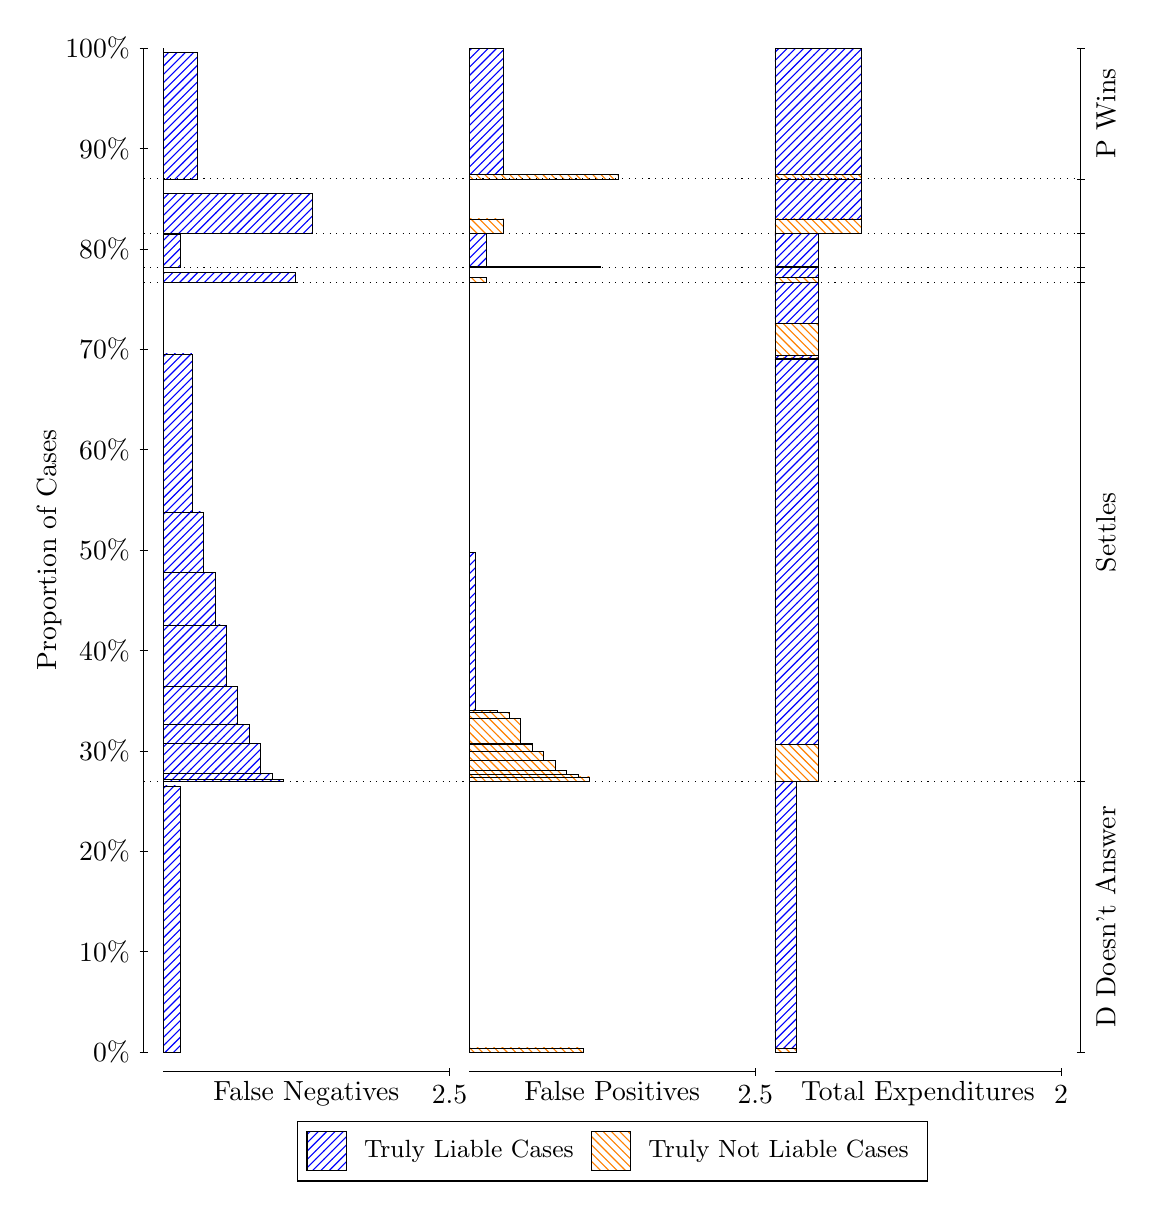
\begin{tikzpicture}
\draw[black, very thin] (1.5,1.75) -- (1.5,14.5);
\node[rotate=90, text=black, anchor=center] at (0.3, 8.125) {Proportion of Cases};
\draw[black, very thin] (1.45,1.75) -- (1.55,1.75);
\node[text=black, anchor=east] at (1.45, 1.75) {0\%};
\draw[black, very thin] (1.45,3.025) -- (1.55,3.025);
\node[text=black, anchor=east] at (1.45, 3.025) {10\%};
\draw[black, very thin] (1.45,4.3) -- (1.55,4.3);
\node[text=black, anchor=east] at (1.45, 4.3) {20\%};
\draw[black, very thin] (1.45,5.575) -- (1.55,5.575);
\node[text=black, anchor=east] at (1.45, 5.575) {30\%};
\draw[black, very thin] (1.45,6.85) -- (1.55,6.85);
\node[text=black, anchor=east] at (1.45, 6.85) {40\%};
\draw[black, very thin] (1.45,8.125) -- (1.55,8.125);
\node[text=black, anchor=east] at (1.45, 8.125) {50\%};
\draw[black, very thin] (1.45,9.4) -- (1.55,9.4);
\node[text=black, anchor=east] at (1.45, 9.4) {60\%};
\draw[black, very thin] (1.45,10.675) -- (1.55,10.675);
\node[text=black, anchor=east] at (1.45, 10.675) {70\%};
\draw[black, very thin] (1.45,11.95) -- (1.55,11.95);
\node[text=black, anchor=east] at (1.45, 11.95) {80\%};
\draw[black, very thin] (1.45,13.225) -- (1.55,13.225);
\node[text=black, anchor=east] at (1.45, 13.225) {90\%};
\draw[black, very thin] (1.45,14.5) -- (1.55,14.5);
\node[text=black, anchor=east] at (1.45, 14.5) {100\%};

\draw[black, very thin] (13.4,1.75) -- (13.4,14.5);
\draw[black, very thin] (13.35,1.75) -- (13.45,1.75);
\node[anchor=west] at (13.35, 1.75) {};
\draw[black, very thin] (13.35,5.1819) -- (13.45,5.1819);
\node[anchor=west] at (13.35, 5.1819) {};
\draw[black, very thin] (13.35,11.52) -- (13.45,11.52);
\node[anchor=west] at (13.35, 11.52) {};
\draw[black, very thin] (13.35,11.716) -- (13.45,11.716);
\node[anchor=west] at (13.35, 11.716) {};
\draw[black, very thin] (13.35,12.143) -- (13.45,12.143);
\node[anchor=west] at (13.35, 12.143) {};
\draw[black, very thin] (13.35,12.838) -- (13.45,12.838);
\node[anchor=west] at (13.35, 12.838) {};
\draw[black, very thin] (13.35,14.5) -- (13.45,14.5);
\node[anchor=west] at (13.35, 14.5) {};

\draw[black, very thin, pattern color=blue, pattern=north east lines] (1.75,1.75) rectangle (1.968,5.1289);
\draw[black, very thin, pattern color=orange, pattern=north west lines] (1.75,5.1289) rectangle (1.75,5.1819);
\draw[black, very thin, pattern color=blue, pattern=north east lines] (1.75,5.1819) rectangle (3.276,5.212);
\draw[black, very thin, pattern color=blue, pattern=north east lines] (1.75,5.212) rectangle (3.1307,5.2885);
\draw[black, very thin, pattern color=blue, pattern=north east lines] (1.75,5.2885) rectangle (2.9853,5.6732);
\draw[black, very thin, pattern color=blue, pattern=north east lines] (1.75,5.6732) rectangle (2.84,5.9087);
\draw[black, very thin, pattern color=blue, pattern=north east lines] (1.75,5.9087) rectangle (2.6947,6.397);
\draw[black, very thin, pattern color=blue, pattern=north east lines] (1.75,6.397) rectangle (2.5493,7.1746);
\draw[black, very thin, pattern color=blue, pattern=north east lines] (1.75,7.1746) rectangle (2.404,7.8406);
\draw[black, very thin, pattern color=blue, pattern=north east lines] (1.75,7.8406) rectangle (2.2587,8.6085);
\draw[black, very thin, pattern color=blue, pattern=north east lines] (1.75,8.6085) rectangle (2.1133,10.616);
\draw[black, very thin, pattern color=orange, pattern=north west lines] (1.75,10.616) rectangle (1.75,11.52);
\draw[black, very thin, pattern color=blue, pattern=north east lines] (1.75,11.52) rectangle (3.4213,11.648);
\draw[black, very thin, pattern color=orange, pattern=north west lines] (1.75,11.648) rectangle (1.75,11.716);
\draw[black, very thin, pattern color=blue, pattern=north east lines] (1.75,11.716) rectangle (1.968,12.135);
\draw[black, very thin, pattern color=orange, pattern=north west lines] (1.75,12.135) rectangle (1.75,12.143);
\draw[black, very thin, pattern color=blue, pattern=north east lines] (1.75,12.143) rectangle (3.6393,12.652);
\draw[black, very thin, pattern color=orange, pattern=north west lines] (1.75,12.652) rectangle (1.75,12.838);
\draw[black, very thin, pattern color=blue, pattern=north east lines] (1.75,12.838) rectangle (2.186,14.444);
\draw[black, very thin, pattern color=orange, pattern=north west lines] (1.75,14.444) rectangle (1.75,14.5);
\draw[black, very thin, pattern color=orange, pattern=north west lines] (5.6333,1.75) rectangle (7.0867,1.8031);
\draw[black, very thin, pattern color=blue, pattern=north east lines] (5.6333,1.8031) rectangle (5.6333,5.1819);
\draw[black, very thin, pattern color=orange, pattern=north west lines] (5.6333,5.1819) rectangle (7.1593,5.2431);
\draw[black, very thin, pattern color=orange, pattern=north west lines] (5.6333,5.2431) rectangle (7.014,5.2773);
\draw[black, very thin, pattern color=orange, pattern=north west lines] (5.6333,5.2773) rectangle (6.8687,5.3229);
\draw[black, very thin, pattern color=orange, pattern=north west lines] (5.6333,5.3229) rectangle (6.7233,5.453);
\draw[black, very thin, pattern color=orange, pattern=north west lines] (5.6333,5.453) rectangle (6.578,5.5705);
\draw[black, very thin, pattern color=orange, pattern=north west lines] (5.6333,5.5705) rectangle (6.4327,5.6547);
\draw[black, very thin, pattern color=orange, pattern=north west lines] (5.6333,5.6547) rectangle (6.4327,5.6734);
\draw[black, very thin, pattern color=orange, pattern=north west lines] (5.6333,5.6734) rectangle (6.2873,5.9854);
\draw[black, very thin, pattern color=orange, pattern=north west lines] (5.6333,5.9854) rectangle (6.142,6.0619);
\draw[black, very thin, pattern color=orange, pattern=north west lines] (5.6333,6.0619) rectangle (5.9967,6.0855);
\draw[black, very thin, pattern color=blue, pattern=north east lines] (5.6333,6.0855) rectangle (5.706,8.0929);
\draw[black, very thin, pattern color=blue, pattern=north east lines] (5.6333,8.0929) rectangle (5.6333,11.52);
\draw[black, very thin, pattern color=orange, pattern=north west lines] (5.6333,11.52) rectangle (5.8513,11.587);
\draw[black, very thin, pattern color=blue, pattern=north east lines] (5.6333,11.587) rectangle (5.6333,11.716);
\draw[black, very thin, pattern color=orange, pattern=north west lines] (5.6333,11.716) rectangle (7.3047,11.724);
\draw[black, very thin, pattern color=blue, pattern=north east lines] (5.6333,11.724) rectangle (5.8513,12.143);
\draw[black, very thin, pattern color=orange, pattern=north west lines] (5.6333,12.143) rectangle (6.0693,12.33);
\draw[black, very thin, pattern color=blue, pattern=north east lines] (5.6333,12.33) rectangle (5.6333,12.838);
\draw[black, very thin, pattern color=orange, pattern=north west lines] (5.6333,12.838) rectangle (7.5227,12.895);
\draw[black, very thin, pattern color=blue, pattern=north east lines] (5.6333,12.895) rectangle (6.0693,14.5);
\draw[black, very thin, pattern color=orange, pattern=north west lines] (9.5167,1.75) rectangle (9.7892,1.8031);
\draw[black, very thin, pattern color=blue, pattern=north east lines] (9.5167,1.8031) rectangle (9.7892,5.1819);
\draw[black, very thin, pattern color=orange, pattern=north west lines] (9.5167,5.1819) rectangle (10.062,5.6547);
\draw[black, very thin, pattern color=blue, pattern=north east lines] (9.5167,5.6547) rectangle (10.062,10.541);
\draw[black, very thin, pattern color=orange, pattern=north west lines] (9.5167,10.541) rectangle (10.062,10.565);
\draw[black, very thin, pattern color=blue, pattern=north east lines] (9.5167,10.565) rectangle (10.062,10.595);
\draw[black, very thin, pattern color=orange, pattern=north west lines] (9.5167,10.595) rectangle (10.062,11.002);
\draw[black, very thin, pattern color=blue, pattern=north east lines] (9.5167,11.002) rectangle (10.062,11.52);
\draw[black, very thin, pattern color=orange, pattern=north west lines] (9.5167,11.52) rectangle (10.062,11.587);
\draw[black, very thin, pattern color=blue, pattern=north east lines] (9.5167,11.587) rectangle (10.062,11.716);
\draw[black, very thin, pattern color=orange, pattern=north west lines] (9.5167,11.716) rectangle (10.062,11.724);
\draw[black, very thin, pattern color=blue, pattern=north east lines] (9.5167,11.724) rectangle (10.062,12.143);
\draw[black, very thin, pattern color=orange, pattern=north west lines] (9.5167,12.143) rectangle (10.607,12.33);
\draw[black, very thin, pattern color=blue, pattern=north east lines] (9.5167,12.33) rectangle (10.607,12.838);
\draw[black, very thin, pattern color=orange, pattern=north west lines] (9.5167,12.838) rectangle (10.607,12.895);
\draw[black, very thin, pattern color=blue, pattern=north east lines] (9.5167,12.895) rectangle (10.607,14.5);
\draw[black, dotted] (1.5,5.1819) -- (13.4,5.1819);
\draw[black, dotted] (1.5,11.52) -- (13.4,11.52);
\draw[black, dotted] (1.5,11.716) -- (13.4,11.716);
\draw[black, dotted] (1.5,12.143) -- (13.4,12.143);
\draw[black, dotted] (1.5,12.838) -- (13.4,12.838);
\draw[black, very thin] (1.75,1.5) -- (5.3833,1.5);
\node[text=black, anchor=north] at (3.5667, 1.5) {False Negatives};
\draw[black, very thin] (5.3833,1.45) -- (5.3833,1.55);
\node[text=black, anchor=north] at (5.3833, 1.45) {2.5};

\draw[black, very thin] (5.6333,1.5) -- (9.2667,1.5);
\node[text=black, anchor=north] at (7.45, 1.5) {False Positives};
\draw[black, very thin] (9.2667,1.45) -- (9.2667,1.55);
\node[text=black, anchor=north] at (9.2667, 1.45) {2.5};

\draw[black, very thin] (9.5167,1.5) -- (13.15,1.5);
\node[text=black, anchor=north] at (11.333, 1.5) {Total Expenditures};
\draw[black, very thin] (13.15,1.45) -- (13.15,1.55);
\node[text=black, anchor=north] at (13.15, 1.45) {2};

\node[text=black, centered, rotate=90] at (13.72, 3.466) {D Doesn't Answer};
\node[text=black, centered, rotate=90] at (13.72, 8.3507) {Settles};



\node[text=black, centered, rotate=90] at (13.72, 13.669) {P Wins};

\draw (7.449999999999999,1.5) node[draw=none] (baseCoordinate) {};
\begin{scope}[align=center]
        \matrix[scale=0.5, draw=black, below=0.5cm of baseCoordinate, nodes={draw}, column sep=0.1cm]{
            \node[rectangle, draw, minimum width=0.5cm, minimum height=0.5cm, pattern color=blue, pattern=north east lines] {}; &
            \node[draw=none, font=\small, text=black] (B) {Truly Liable Cases}; &
            \node[rectangle, draw, minimum width=0.5cm, minimum height=0.5cm, pattern color=orange, pattern=north west lines] {}; &
            \node[draw=none, font=\small, text=black] (B) {Truly Not Liable Cases}; \\
            };
\end{scope}

\end{tikzpicture}
\end{document}